\documentclass[../main.tex]{subfiles}
\begin{document}
Un circuito logico è composto da $n$ input e $m$ output (non c'è solo un ouput come per le porte logiche). Inoltre al suo interno
possonoo esserci dei circuiti, ogni circuito è un elemento.
\begin{figure}[h]
    \centering
    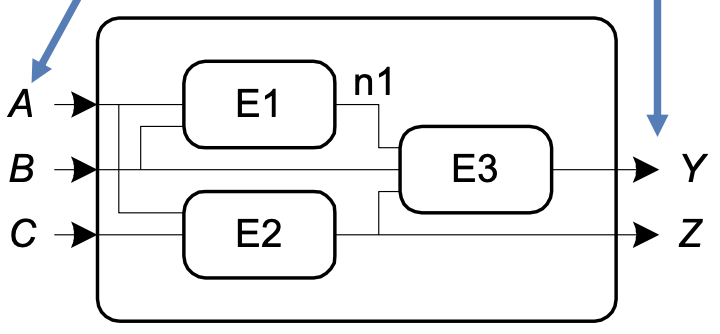
\includegraphics[width=0.5\textwidth]{images/circuitoLogico.png}
\end{figure}

Esistono due tipi di circuiti logici:
\begin{itemize}
    \item \textbf{Logica combinazionale (CL)}, non ha memoria, l'output è determinato solo dagli input
    \item \textbf{Logica sequenziale}, ha memoria, l'output è determinato anche dagli input precedenti
\end{itemize}

Per ora concentriamoci sui circuiti con \textbf{logica combinazionale}, ogni elemento di questo tipo di circuito deve essere
anch'esso combinazionale. Inoltre ogni nodo di un circuito combinazionale è collegato sia a un ingresso che a un uscita.

\subsection{Algebra booleana}
Alcune definizioni:
\begin{itemize}
    \item \textbf{Complemento}: una viariabile "negata", $\bar{A}, \bar{B}, \bar{C}$
    \item \textbf{Letterale}: una viariabile o il suo complemento, $A, \bar{A}, B, \bar{B}, C, \bar{C}$
    \item \textbf{Implicante}: il prodotto di due o più letterali, $AB\bar{C}, A\bar{B}, BC$
    \item \textbf{Minterm}: un implicante che inlcude \underline{tutte} le variabili di input esattamente una volta, $AB\bar{C}, A\bar{B}\bar{C}, ABC$
    \item \textbf{Maxterm}: la \underline{somma} che include \underline{tutte} le variabili di input esattamente una volta, $(A+\bar{B}+C), (\bar{A}+B+\bar{C}), (\bar{A}+\bar{B}+C)$
\end{itemize}
\textbf{Nota:} $(A+\bar{B}+\bar{A}+C)$ non è \textbf{Maxterm} perchè l'input $A$ c'è due volte, anche se una di queste è negato.

Di seguito è riportata una tabella con tutti i teoremi e gli assiomi che possiamo utilizzare:
\begin{figure}[h]
    \centering
    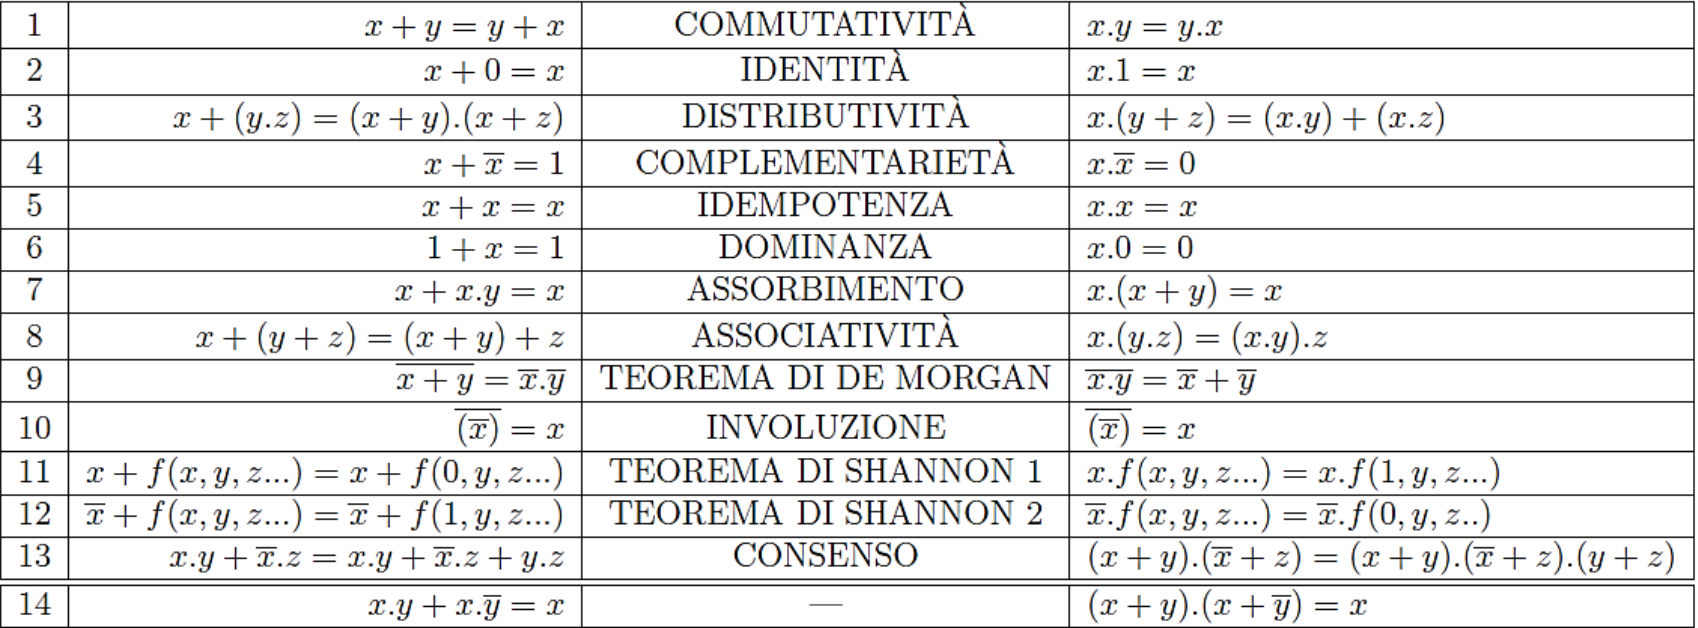
\includegraphics[width=1\textwidth]{images/teoremiAlgebraBool.png}
    \caption{Proprietà e teoremi dell'algebra di Boole}
\end{figure}

\pagebreak
\subsubsection{Somma dei prodotti}
La \textbf{SOP} (Sum-of-Products) è una forma nella quale possiamo scrivere una qualsiasi equazione booleana utilizzando i \textbf{minterm}.
$$
    Y = F(A,B) = \sum_{i = 0}^{n}(mi)\phantom{--};n=2^N -1 
$$
Guardiamo un esempio per capire come utilizzarala:
\begin{figure}[h]
    \centering
    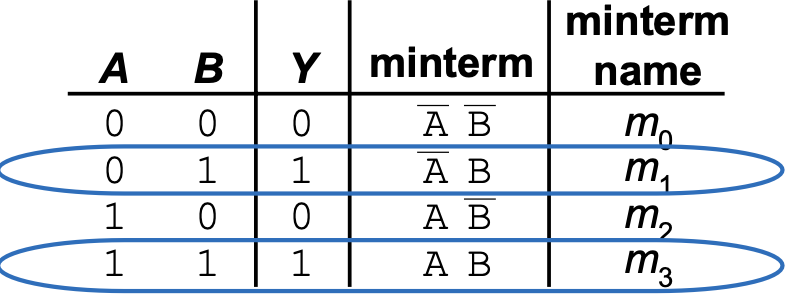
\includegraphics[width=0.5\textwidth]{images/sop.png}
\end{figure}

In questo caso
$$
    Y = F(A,B) = \bar{A}B + AB = \sum(1,3)
$$

\subsubsection{Prodotto delle somme}
La \textbf{POS} (product-of-Sums) è una forma nella quale possiamo scrivere qualsiasi equazione booleana utilizzando i \textbf{maxterm}.
$$
    Y = F(A,B) = \prod_{i = 0}^{n}(Mi)\phantom{--};n=2^N  -1
$$
Guardiamo un esempio per capire come utilizzarala:
\begin{figure}[h]
    \centering
    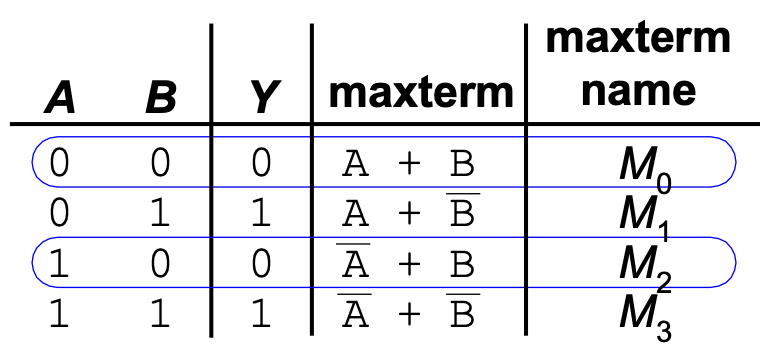
\includegraphics[width=0.5\textwidth]{images/pos.png}
\end{figure}

In questo caso
$$
    Y = F(A,B) = (A+B)(\bar{A}+B) = \prod(0,2)
$$

\pagebreak
\subsubsection{Teorema di DeMorgan}
$$
    Y = \bar{AB} = \bar{A} + \bar{B}
$$
\begin{figure}[h]
    \centering
    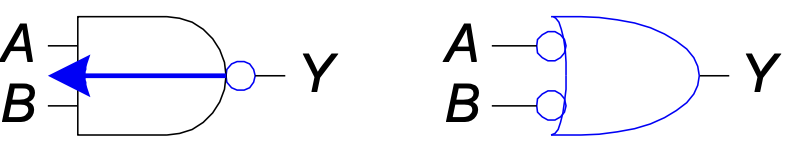
\includegraphics[width=0.4\textwidth]{images/bubbleBackward.png}
\end{figure}

ma anche
$$
    Y = \bar{A+B} = \bar{A} \cdot \bar{B}
$$
\begin{figure}[h]
    \centering
    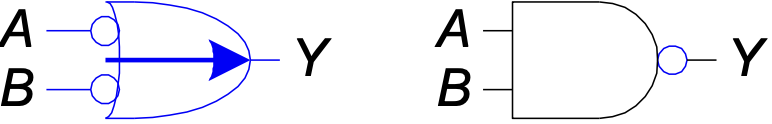
\includegraphics[width=0.4\textwidth]{images/bubbleForward.png}
\end{figure}

Queste operazioni sono anche conosciute come \textbf{bubble pushing}. Esso si applica preferibilmente in modo tale che l'entrata 
sia uguale all'uscita. In altre parole se l'output è negato preferibilmente vogliamo avere anche l'input sucessivo negato in modo tale 
che sia facile semplificare l'espressione booleana.
% Vedi slide 37 se hai dubbi


\subsection{Da espressione a porte logiche}
Per passare da un espressione booleana ad uno schema logico seguiamo degli step:
\begin{enumerate}
    \item Scriviamo tutti i letterali presenti nella funzione
    \item Scriviamo le espressioni intermedie
    \item Colleghiamo i letterali rendendo le espressioni coerenti
    \item Scriviamo l'output
\end{enumerate}
%Vedi slide 38 se hai dubbi


In generale durante la creazione di uno schema seguiamo le seguenti pratiche:
\begin{itemize}
    \item I letterali (gli input) vanno scritti sulla sinistra o nella parte superiore
    \item Gli output vanno scritti sulla destra o sulla parte inferiore
    \item Il flusso delle porte va da sinistra verso destra
    \item Le linee devono essere preferibilmente dritte
    \item La giunzione di più cavi è rappresentata con un punto (i cavi che si intersecano senza punto non sono connessi)
\end{itemize}

\pagebreak
\subsection{Circuito prioritario}
In questo tipo di circuito viene considerato solo il bit più significativo (\textbf{MSB}), in caso di più input con valore \code{1}
viene considerato per l'output solo quello con MSB maggiore. Nella tabella della verità ci sarà sempre un solo 
bit con valore \code{1} per riga:
\begin{figure}[h]
    \centering
    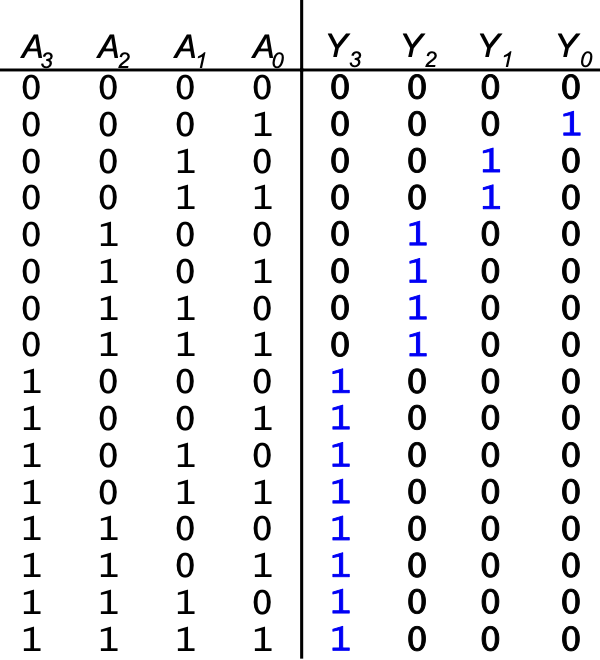
\includegraphics[width=0.4\textwidth]{images/circuitoPrioritario.png}
\end{figure}

\subsection{Don't Cares}
Don't Cares è una tabella della verità che esclude i valori "inutili" di un'altra tabella della verità analoga. Nel caso del circuito
prioritario la tabella sarebbe:
\begin{figure}[h]
    \centering
    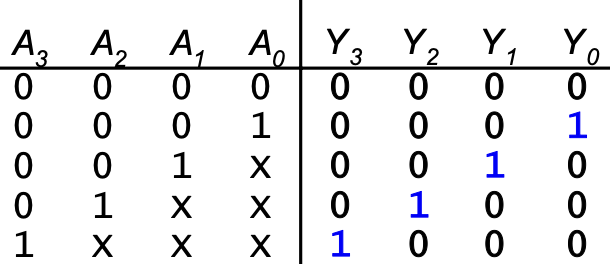
\includegraphics[width=0.4\textwidth]{images/dontCares.png}
\end{figure}

I don't cares vengono usati per semplificare i circuiti, decidiamo noi il criterio ma solitamente li usiamo per situazioni che non
possono verificarsi.
% Vedi slide 45 se hai dubbi

\pagebreak
\subsection{Mappe di Karnaugh}
\subsubsection{Grey code}
Il Grey Code è una rappresentazione alternativa per i numeri binari:
\begin{figure}[h]
    \centering
    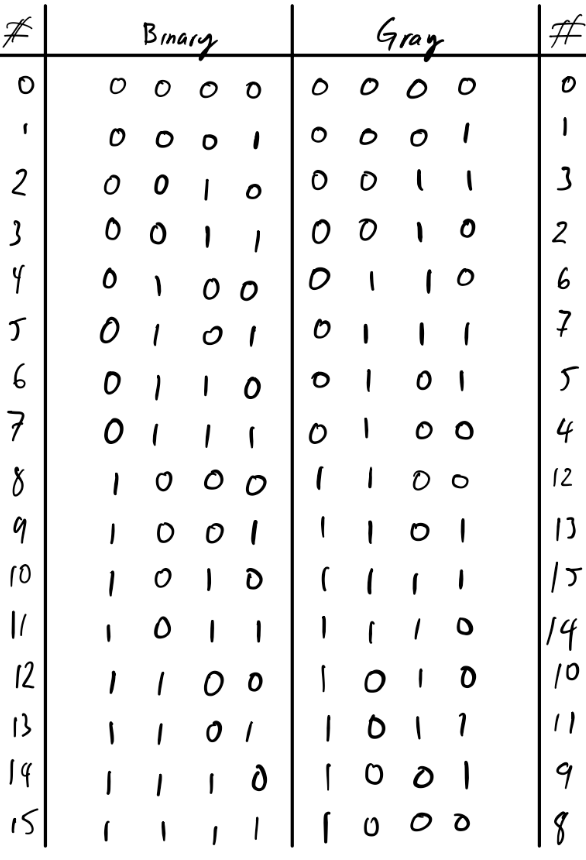
\includegraphics[width=0.4\textwidth]{images/grayCode.png}
\end{figure}

\subsubsection{Come creare una mappa}
Data una funzione
$$
    Y = f(A, B, C, D)
$$
la sua mappa di Karnaugh si costruisce facendo una tabella contenente $2^n$ colonne, dove $n$ è il numero di input per la parte superiore
e $2^m$ righe, dove $m$ è ikl numero di input per la parte inferiore.

\textbf{Nota:} la scelta di quanti e quali input usare per le righe e per le colonne è libera.
% Vedi immagine a slide 53 e 54

Ad ogni casella inoltre corrisponde una combinazione di Grey Code per le righe e una per le colonne. Il valore delle caselle è dato
dalla combinazione di questi codici. La struttura consigliata per questo tipo di mappa è di \textbf{massimo 4 input}.
\begin{figure}[h]
    \centering
    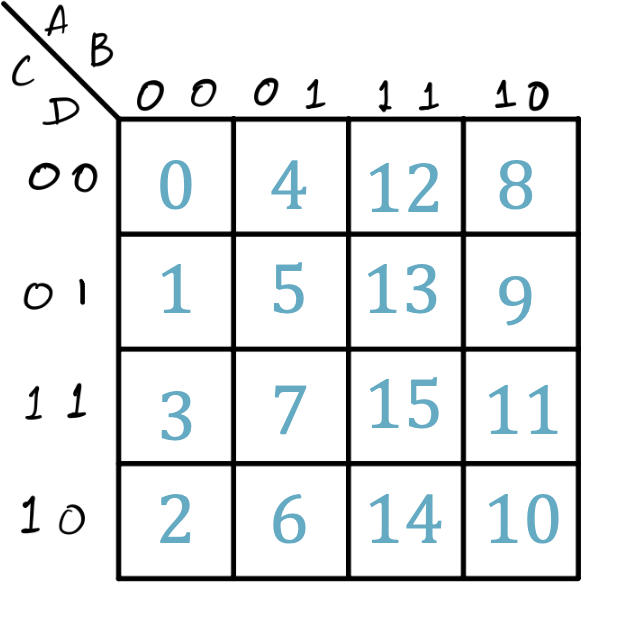
\includegraphics[width=0.4\textwidth]{images/karnaugh.png}
\end{figure}

\subsubsection{Come usare una mappa}
Possiamo utilizzare queste mappe per risolvere graficamente una funzione booleana. Sostituendo i valori del Grey Code con gli input e gli
input negati della funzione possiamo facilmente stabilire dei pattern nella mappa per i \textbf{SOP} o i \textbf{POS} (casi più comuni).
% Vedi da slide 64 a 68

\vspace{1cm}
\subsubsection{Da tabella della verità a mappa}
\begin{figure}[h]
    \centering
    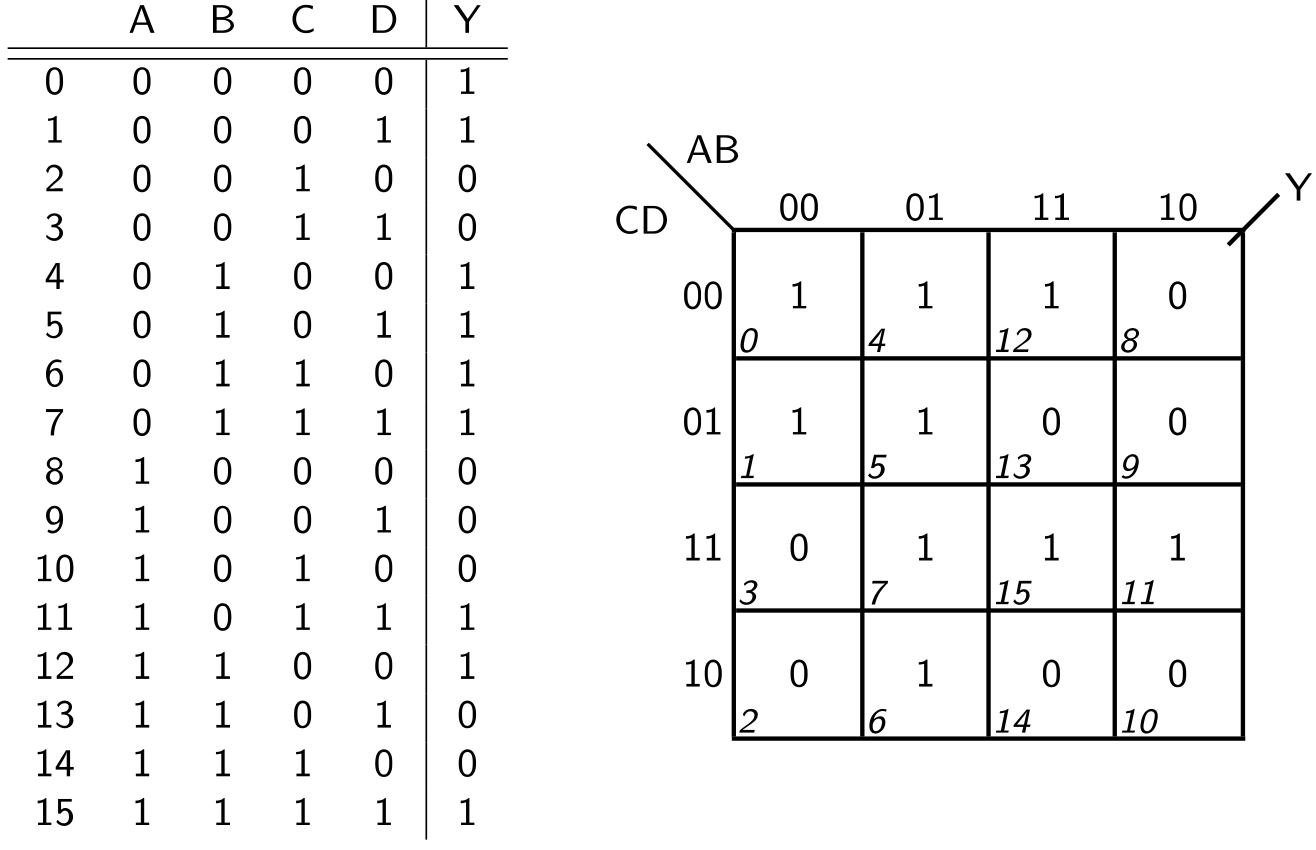
\includegraphics[width=0.6\textwidth]{images/tabellaMappa.png}
\end{figure}

\vspace{1cm}
\subsubsection{Formare i gruppi}
Possiamo utilizzare una mappa di Karnaugh per trovare dei pattern. In generale due caselle adiacenti hanno sempre e solo un bit di
differenza e sono quelle che quindi possono essere ragggruppate. Bisogna sempre cercare di fare \underline{meno gruppi possibili}, 
prendendo quindi le \underline{combinazioni più grandi possibili}.
\begin{figure}[h]
    \centering
    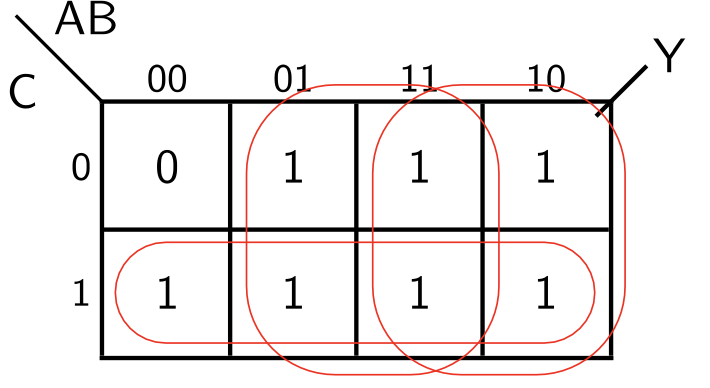
\includegraphics[width=0.4\textwidth]{images/gruppi.png}
\end{figure}

Ogni gruppo formato rappresenta un'espressione booleana, se abbiamo formato correttamente i gruppi esse si semplificano ad un solo letterale.
La funzione finale semplificata al massimo sarà l'unione dei letterali restituiti da ogni singolo gruppo.

\textbf{Nota:} la soluzione finale della funzione non è univoca, potrebbero esserci più soluzioni valide semplificate al massimo prendendo
ad esempio gruppi diversi.l
% Vedi da slide 77 a 79

\pagebreak
\subsection{Metodo Quine-McClusky}
Il metodo Quine-McClusky è un algoritmo alternativo alla mappa di Karnaugh, lo si preferisce quando abbiamo più di 4 input. 
Per applicare McClusky bisogna partire da una specifica situazione iniziale:
\begin{enumerate}
    \item Partire dalla forma canonica di una funzione (SOP o POS)
    \item 
\end{enumerate}

\subsubsection{Peso e distanza}
$$
    HD(XY) = w(X\oplus Y)
$$
\begin{itemize}
    \item $HD$ indica la distanza tra due parole binarie, ovvero la quantità di \code{bit} differenti tra loro
    \item $w$ indica il peso di una parola binaria, ovvero quanti \code{bit} sono $1$
\end{itemize}

\subsubsection{Esempio}
Facciamo ora un esempio dove applichiamo il metodo McClusky. Supponiamo di voler minimizzare la funzione
$$
    F(A,B,C,D) = \underbrace{\sum m(4,5,6,8,9,10,13)}_{\text{ON - Set}} + \underbrace{\sum d(0,7,15)}_{\text{DC - Set}}
$$

\vspace{0.2cm}
\begin{enumerate}
    \item Riempire la colonna 1 con i \underline{MIN termini} di ON-set e DC-set raggruppati in base al loro peso
    \item Confrontare gli elementi dei gruppi adiacenti alla ricerca di termini a distanza 1. Eliminare la variabile e mettere nella
    colonna successiva. \textit{es.} $0000$ e $0100 \Rightarrow 0-00$. 

    Segnare con \checkmark i termini che ne generano uno più semplice. Se non generano altri termini segnare con \textit{IP} (\textbf{Implicante Primo}).
    
    \textbf{Nota:} ripetere questo step finchè non si possono avere più combinazioni.
    \item Creare la tabella di copertura che permette di trovare la collezione minima di \textbf{IP} che copre l'ON-set.
\end{enumerate}
% Vedi da slide 111 a 161 :)


\end{document}